\chapter{Introducción}

\label{cap:introduccion}
Este Trabajo de Fin de Máster presenta el diseño e implementación de un sistema completo de adquisición, transmisión y visualización de datos en tiempo real inspirado en el concepto CanSat.
El proyecto está formado por la construcción de un dispositivo tipo CanSat, con diferentes sensores, GPS, cámara y comunicación por wifi o radio,
además, una plataforma web opensource encargada de visualizar los datos recogidos en tiempo real.
Esta plataforma se ha diseñado como una herramienta genérica y reutilizable de forma que se pueda adaptar fácilmente a otros proyectos similares.
A lo largo del documento se describen el contexto del trabajo, la motivación, los objetivos planteados, la planificación seguida y la estructura de la memoria.

\begin{figure}
    \centering
    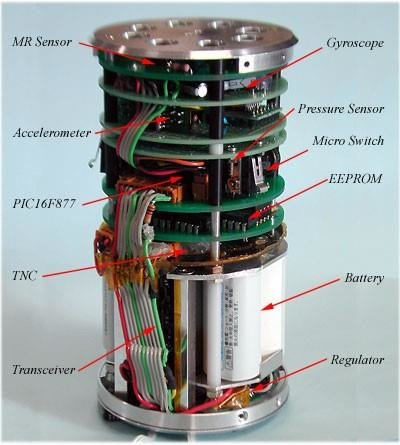
\includegraphics[width=0.5\textwidth]{Imagenes/Bitmap/cansat}
    \caption{Diagrama básico de un CanSat. Fuente: \cite{researchgate_cansat2018}}
    \label{fig:cansat}
\end{figure}


\section{Contexto}
El proyecto CanSat propuesto por el profesor Robert J. Twiggs en 1998~\cite{jaxa_cansat} comienza como un proyecto educativo basado en la simulación de un nanosatélite del tamaño de una lata de refresco y de un peso alrededor de los 350 gramos,
el objetivo es ayudar a los alumnos de distintos niveles a entender todas las fases de desarrollo de un satélite, desde la elección de la misión científica hasta la integración del sistema completo,
incluyendo los sensores necesarios para obtener los datos necesarios para dicha misión, la electronica necesaria para usar dichos sensores y enviarlos por radio a una estación de tierra,
la visualización de los datos, el diseño de una carcasa 3d capaz de aguantar la fuerza del lanzamiento y el diseño de un paracaídas.

Los CanSat no son puestos en órbita, pero son lanzados por cohetes a escala, globos aerostáticos o drones,
esto los somete a distintas fuerzas externas como aceleración, vibraciones o posibles impactos, lo que hace que el CanSat tenga que tener una estructura resistente.
La misión del CanSat es usar los sensores para recoger datos durante el descenso y transmitirlos a la estación de tierra.

Durante los últimos años la popularidad del proyecto ha ido aumentando, llegando a crear competiciones nacionales e internacionales lideradas por agencias espaciales como la agencia espacial europea~\cite{esa_cansat2024}
con el objetivo de promover el interés por el sector aeroespacial y por las carreras STEM en general desde pequeños.


\section{Motivación}
Debido a que estos proyectos suelen estar más enfocados en la parte electronica(recogida y transmisión de datos) y no tanto en la visualización de datos,
esta última parte suele quedar más descuidada, implementandose solo soluciones básicas como visualización de datos por consola o gráficas simples.
Además, estas soluciones son específicas para un CanSat concreto, lo que obliga a implementar soluciones desde cero.

Por ello, surge la necesidad de crear una plataforma común y reutilizable que permita visualizar en tiempo real los datos enviados por el CanSat y recibidos por la antena de manera más visual y profesional sin depender de un hardware concreto.
Con la creación de esta plataforma se facilitaría el análisis de los datos durante las pruebas y el lanzamiento,
además puede servir como base para futuras implementaciones específicas, ayudando a que los alumnos integren gráficas avanzadas sin tener que desarrollar una plataforma completa.


\section{Objetivos}
El objetivo principal de este proyecto consiste en diseñar y desarrollar desde cero un satélite tipo CanSat y la implementación una plataforma de visualización de datos reutilizable.
Para ello se han dividido los objetivos en dos partes diferenciadas: investigación de las tecnologías actuales y desarrollo del CanSat.

\begin{itemize}
    \item \textbf{Investigación}
    \begin{itemize}
        \item Comparación de los distintos microcontroladores y microcomputadores existentes para determinar cuál se ajusta mejor a los objetivos de nuestro desarrollo.
        \item Estudio de los distintos sensores disponibles en el mercado y su comunicación con el microcomputador.
        \item Análisis de las diferentes opciones de alimentación para el CanSat y de la posibilidad de cargarse con paneles solares.
        \item Comparación de las herramientas actuales de visualización de datos.
    \end{itemize}
    \item \textbf{Desarrollo}, dividido en dos partes: la creación del hardware del CanSat y la plataforma de visualización.
    \begin{itemize}
        \item CanSat
        \begin{itemize}
            \item Creación de un CanSat que cumpla con las medidas básicas (66mm x 115mm) y peso (entre 300g y 350g).
            \item Integración de receptor GPS
            \item Cámara para transmisión de video en tiempo real.
            \item Sensor de presión, temperatura y altitud.
            \item Giroscopio para obtener la orientación del dispositivo.
            \item Batería con posibilidad de carga mediante paneles solares.
            \item Retransmisión de los datos por WIFI si el dispositivo tiene conexión a internet.
            \item Retransmisión de los datos por radio en caso de que no tenga conexión.
            \item Desarrollo de un receptor de radio en la estación terrestre.
        \end{itemize}
        \item Plataforma de visualización
        \begin{itemize}
            \item Visualización en tiempo real de toda la telemetría recibida.
            \item Visualización del último valor de cada elemento de la telemetría.
            \item Gráficas en tiempo real de los valores recibidos.
            \item Visualización en tiempo real de las imágenes transmitidas.
            \item Mapa con la ubicación exacta del CanSat.
            \item Modelo 3D con la orientación real del CanSat.
            \item Descarga de los datos de telemetría para un rango de fechas concreto.
        \end{itemize}
    \end{itemize}
\end{itemize}


\section{Plan de trabajo}
Durante el desarrollo del proyecto se ha seguido un plan de trabajo con el objetivo de organizar las tareas y alcanzar los objetivos mencionados anteriormente.
Este plan de trabajo se ha dividido en los siguientes puntos:

\begin{itemize}
    \item Revisión y comparación de los microprocesadores Arduino y ESP32 y del microcomputador Raspberry Pi Zero 2 en función de sus capacidades y compatibilidad con los sensores y módulos de comunicación.
    \item Selección de los sensores (GPS, altímetro y giroscopio), módulo de comunicación (LoRa), cámara y sistema de alimentación.
    \item Ensamblaje inicial de los distintos componentes electrónicos usando placas de prototipado, lo que facilita las pruebas individuales de cada componente.
    \item Definición de la arquitectura general del sistema compuesta por tres componentes principales:
    \begin{itemize}
        \item Código embebido en la Raspberry Pi encargado de leer los sensores y transmisión de datos.
        \item Receptor de radio en tierra encargado de la recepción de los datos enviados por el CanSat.
        \item Plataforma de visualización en tiempo real.
    \end{itemize}
    \item Implementación del código embebido en la Raspberry usando Python y las distintas librerías para interactuar con cada sensor.
    \item Implementación de la plataforma de visualización en tiempo real basada en eventos, usando un sistema de colas RabbitMQ, un backend en Java y Spring Boot, un frontend en Flutter y una base de datos PostgreSQL para guardar los datos de telemetría.
    \item Soldar los componentes electrónicos en una placa definitiva de un tamaño que cumpla con las medidas reglamentarias de CanSat.
    \item Realización de pruebas de integración una vez todo el sistema esté terminando, incluyendo pruebas de duración de batería y de alcance de comunicaciones por radio.
    \item Redacción de la memoria documentando los pasos seguidos en el proyecto y los resultados obtenidos.
\end{itemize}


\section{Organización de la memoria}

La memoria se compone de los siguientes capítulos:

\begin{itemize}
    \item \textbf{Capítulo 1. Introducción:} se presenta el contexto del proyecto, la motivación personal y académica, los objetivos planteados y el plan de trabajo seguido.

    \item \textbf{Capítulo 2. Trabajo relacionado:} se revisan iniciativas previas relacionadas con el concepto CanSat, tanto en el ámbito educativo como técnico, y se analizan distintas soluciones de adquisición, transmisión y visualización de datos.

    \item \textbf{Capítulo 3. Fundamentos teóricos:} se definen los conceptos técnicos necesarios para el desarrollo del sistema, incluyendo comparativas de hardware, tecnologías de comunicación, sensores, protocolos de vídeo y arquitecturas de visualización en tiempo real.

    \item \textbf{Capítulo 4. Diseño e implementación del sistema:} se describe la arquitectura del sistema completo, los componentes elegidos, el montaje del CanSat, el desarrollo del software embebido, el backend, el frontend y las pruebas realizadas.

    \item \textbf{Capítulo 5. Conclusiones y trabajo futuro:} se recogen las principales conclusiones del trabajo, se valoran los resultados obtenidos y se proponen posibles mejoras y líneas de desarrollo futuras.
\end{itemize}